\chapter{METODOLOGÍA DE LA INVESTIGACIÓN}
\section{Diseño de la investigación}
En esta sección del documento se explicará cual es el diseño, el tipo y el enfoque del trabajo de investigación, así como también la población y la muestra del estudio. 
%Para finalizar se explicará el
%proceso de aplicación de las redes neuronales convolucionales.
\subsection{Enfoque}
Esta investigación adopta un enfoque cuantitativo, centrado principalmente en el análisis de datos históricos y la aplicación de modelos de series temporales para abordar la demanda de productos perecibles. La metodología se basa en la recopilación y análisis de datos cuantitativos diarios relacionados con la demanda, con el objetivo de ofrecer información y recomendaciones basadas en rigor estadístico y en la interpretación de patrones numéricos. Esto permitirá optimizar la gestión de la demanda de productos y mejorar la eficiencia operativa en la toma de decisiones de inversión en los pedidos a proveedores.

\subsection{Alcance}
Esta investigación es de tipo explicativa, ya que busca identificar los componentes y parámetros específicos que afectan la eficiencia de la cadena de suministro de la empresa Market Donna SAC. En particular, se centrará en el desarrollo e implementación de un sistema de pronóstico de demanda basado en modelos de Forecasting. El alcance se extiende a la evaluación del impacto de este sistema en la gestión de las órdenes de productos perecibles, analizando los beneficios en términos de optimización de inversión, reducción de costos y mejora de la eficiencia operativa.

\subsection{Tipo}
La investigación es de tipo no experimental, dado que se trabajará con datos históricos comprendidos entre el año 2012 Y 2026. A partir de este análisis, se desarrollará un modelo predictivo para mejorar la precisión en la estimación de la demanda de productos en Market Donna SAC y, así, orientar decisiones más efectivas. 

%\subsection{Enfoque cuantitativo}




%%%%%%%%%%%%%%%%%%%%%%%%%%%%%%%%%%%

\subsection{Población y muestra}

La población de estudio incluye todas las categorías de productos que Market Donna SAC ofrece, entre las cuales se encuentran artículos de limpieza, frutas, verduras, lácteos, carnes, bebidas, abarrotes, tabaco, condimentos, embutidos, panes, entre otros. En total, la empresa cuenta con 16 categorías de productos que generan un promedio de 136,000 soles mensuales en ventas.
La muestra seleccionada se concentra específicamente en la categoría de Verduras, que representa una de las familias de productos con mayor impacto en las ventas de la empresa. Al centrarnos en esta categoría de productos perecibles, el estudio busca realizar un análisis más preciso de la demanda diaria y proyectar las ventas en soles para la familia de verduras, dada su relevancia en las operaciones y en la rentabilidad de Market Donna SAC.


\subsection{Unidad de análisis}
La unidad de análisis de este estudio se centra en cada transacción individual de venta de productos dentro de la categoría seleccionada, que corresponde a las verduras. Cada transacción registrada en este segmento, desde el año 2012 hasta 2026, se considera como una unidad única de observación. Esto permite una comprensión granular y precisa de los patrones de compra, comportamientos de los clientes y tendencias de demanda asociadas específicamente a estos productos perecibles.
Al examinar cada transacción de manera individual, el análisis busca capturar variaciones diarias en la demanda, observar los patrones de consumo recurrentes y detectar posibles picos o caídas en las ventas. Este enfoque detallado proporciona información valiosa para construir un modelo predictivo ajustado a las particularidades de la categoría de verduras, permitiendo identificar factores que podrían influir en la demanda, como la estacionalidad, días de la semana, campañas promocionales o eventos externos.
Además, el análisis de estas transacciones ofrece la oportunidad de estudiar la sensibilidad de la demanda a las variaciones en precios y promociones dentro de esta categoría. Estos datos permitirán una mejor previsión de la demanda en soles y servirán de base para la toma de decisiones estratégicas sobre los volúmenes de compra y la inversión diaria en reposición de inventario, asegurando así la disponibilidad de productos frescos y optimizando la eficiencia operativa de Market Donna SAC en esta categoría de productos perecibles.


%La Figura \ref{fig1} y el Cuadro \ref{tab:widgets}
%
%	\begin{figure}[h]
	%		\begin{center}
		%			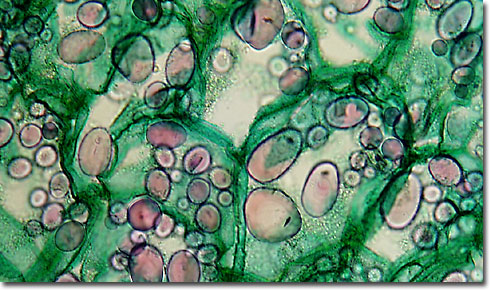
\includegraphics[width=0.8\textwidth]{3/figures/largepotato.jpg}
		%			\caption{Prueba de Figura}
		%			\label{fig1}
		%		\end{center}
	%		
	%	\end{figure}


%\subsection{Operacionalización de Variables}
%
%
%\begin{longtable}{L{2.7cm} | L{4cm} | C{2cm} | C{2.5cm} }
%	\hline
%	\caption{Matriz de operacionalización de variables}
%	%\rowcolor{Gainsboro!60}
%	%\rowcolor{Gray}
%	\makecell{Variable} & \makecell{Definición \\ operacional}  & \makecell{Indicador} & \makecell{Fórmula}\\
%	\hline
%	\endhead
%	Independiente: Optimización en la toma de decisiones & Cantidad óptima de pedidos a realizar a los proveedores, con el fin de minimizar los costos operativos y los desperdicios, al mismo tiempo que se maximiza la disponibilidad de productos y se mejora la eficiencia del inventario  & Cantidad óptima de pedidos & pedido\ proveedor\ <\ demanda\\
%	\hline
%%	Dependiente: Demanda de productos & Cantidad específica de productos que se espera que los consumidores compren en un período de tiempo determinado, basada en datos históricos de ventas & Cantidad de productos & Número de pedidos \le Demanda\\
%%	\hline
%%	\multirow{4}{*}{Modelo \\ de regresión} & \multirow{4}{*}{Modelo con la capacidad de predecir la cantidad aproximada de demanda de productos}  & MSE & \\
%	
%	& & RMSE & \\
%	
%	& & R2 & \\	
%	
%	& & ACCURACY & \\
%	
%	\newline
%	\newline \textit{Fuente: Elaboración propia}
%	\label{tab:widgets}
%\end{longtable}




%%%% TABLA

%\begin{table}[H]
%	\centering
%	\begin{tabular}{|L{2.7cm}|L{4cm}|C{1.9cm}|C{2.5cm}|}
	%		\hline
	%		Variable & Definición operacional & Indicador & Fórmula\\
	%		\hline
	%		Independiente: Optimización en la toma de decisiones & Cantidad óptima de pedidos a realizar a los proveedores, con el fin de minimizar los costos operativos y los desperdicios, al mismo tiempo que se maximiza la disponibilidad de productos y se mejora la eficiencia del inventario & Cantidad óptima de pedidos & Fórmula 1  \\
	%		\hline
	%		Dependiente: Demanda de productos & Cantidad específica de productos que se espera que los consumidores compren en un período de tiempo determinado, basada en datos históricos de ventas & Cantidad de productos & Fórmula 2  \\
	%		\hline
	%		\multirow{3}{*}{Modelo de \\ regresión} & \multirow{3}{4cm}{Modelo con la capacidad de predecir la cantidad aproximada de demanda de productos} & \multirow{2}{*}{Combinadas} & Fórmula 3 \\
	%		\cline{2-2} \cline{4-4}
	%		& & & Fórmula 4 \\
	%		\cline{2-4}
	%		& & Indicador extra & Fórmula 5 \\
	%		\hline
	%	\end{tabular}
%	\caption{Tabla simple}
%\end{table}


%	\begin{table}[ht]
	%	\centering
	%	\begin{tabular}{|c|l|c|r|m{4cm}|}
		%		\hline
		%		Columna 1 & Columna 2 & \multicolumn{2}{c|}{Columna Combinada} & Columna con P\'arrafo\\
		%		\hline
		%		\hline
		%		Fila 1 & Celda 11 & Celda 12 & Celda 13 & Este es un párrafo de muestra en la primera celda de la última columna \\
		%		\hline
		%		\rowcolor{skyblue6}
		%		Fila 2 & Celda 21 & Celda 22 & Celda 23 & Celda P\'arrafo 24 \\
		%		\hline
		%		\parbox[t]{2mm}{\multirow{3}{*}{\rotatebox[origin=c]{90}{Fila 3}}} & Celda 31 & \multirow{2}{*}{Celdas Combinadas} & Celda 33 & Celda P\'arrafo 34  \\
		%		\cline{2-2} \cline{4-5}
		%		& Celda 41 & & Celda 43 & Celda P\'arrafo 44 \\
		%		\cline{2-5}
		%		& Celda 51 & Celda 52 & Celda 53 & Celda P\'arrafo 54  \\
		%		\hline
		%	\end{tabular}
	%	\caption{Tabla simple}
	%\end{table}
	
	%\section{Instrumentos de medida}
	%Nisi porta lorem mollis aliquam ut porttitor leo. Aenean pharetra magna ac placerat \begin{itemize}
		%	\item muscle and fat cells remove glucose from the blood,
		%	\item cells breakdown glucose via glycolysis and the citrate cycle, storing its energy in the form of ATP,
		%	\item liver and muscle store glucose as glycogen as a short-term energy reserve,
		%	\item adipose tissue stores glucose as fat for long-term energy reserve, and
		%	\item cells use glucose for protein synthesis.
		%\end{itemize}
		
		\section{Técnicas de recolección de datos}
		La recolección de datos para esta investigación se focalizó en la obtención de información sobre la categoría de verduras, la cual representa en promedio el 33 \% de la demanda diaria en Market Donna SAC. Esta categoría fue seleccionada estratégicamente debido a su relevancia en la demanda diaria y su corta vida útil, lo que la convierte en un componente esencial para el análisis de productos en la empresa.
		Para implementar el modelo de series de tiempo y realizar pronósticos de demanda diarios que contribuyan a maximizar los ingresos, se llevó a cabo una recopilación exhaustiva de datos históricos a través de un sistema de administración de bases de datos en SQL Server. Inicialmente, se desarrollaron consultas SQL específicas \ref{fig:querysql} para filtrar y extraer las tablas relevantes, tales como las de productos, precios, familias y códigos. Este proceso permitió estructurar y organizar la información de manera adecuada para su posterior análisis.
		Posteriormente, se diseñó una consulta SQL \ref{fig:tablasql} avanzada que integró y combinó las tablas requeridas, garantizando la coherencia e integridad de los datos necesarios para construir los modelos de pronóstico de demanda. Esta metodología proporcionó un conjunto de datos preciso y completo, indispensable para la aplicación de técnicas avanzadas de series de tiempo.
		El análisis incluyó el examen detallado de transacciones de productos de la categoría de verduras desde el año 2012 hasta 2026, brindando una perspectiva temporal amplia para identificar patrones y tendencias de demanda diaria a lo largo del tiempo. Además, se utilizó el sistema de punto de venta (POS) de la empresa para capturar datos en tiempo real sobre las transacciones, lo que permitió un seguimiento constante y detallado de la demanda en esta categoría.
		Para mejorar la precisión de los datos, se revisaron registros continuos de los niveles de inventario de la categoría de verduras. Aunque la investigación se centra en la demanda y no en la gestión de inventarios, este seguimiento indirecto permitió observar cómo la demanda afecta la reposición de productos perecibles, lo cual es crucial para la planificación diaria en productos de alta rotación.
		Estas estrategias de recolección de datos se diseñaron para ofrecer una visión integral y cuantitativa de la demanda de la categoría de verduras en Market Donna SAC, focalizándose en este grupo de productos que tiene un impacto significativo en las ventas diarias y en la eficiencia operativa general de la empresa.
		
		
		
		\begin{figure}[H]
			\begin{center}
				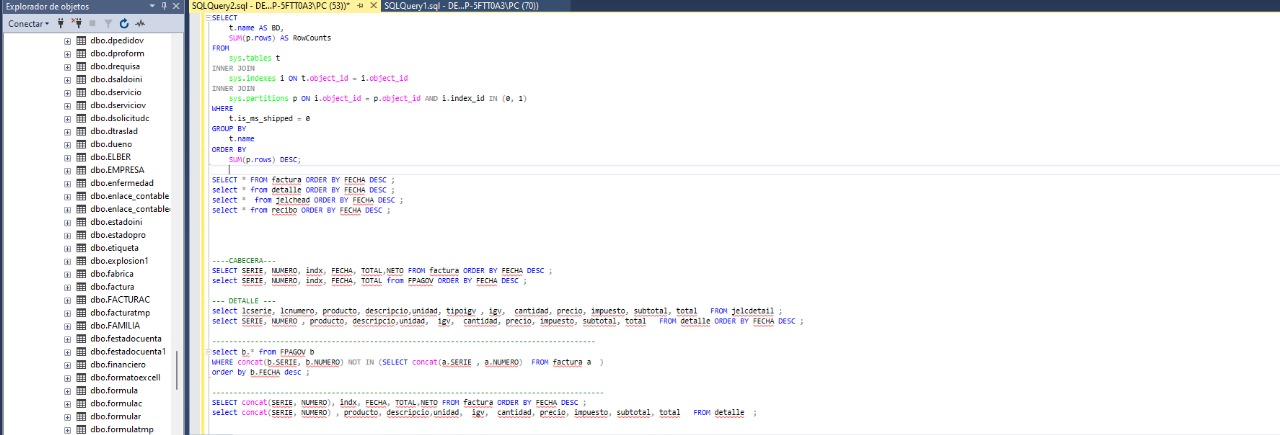
\includegraphics[width=0.9\textwidth]{3/figures/querysql.jpg}
				\caption{Consulta SQL}
				\textit{Fuente: Elaboración propia}
				\label{fig:querysql}
			\end{center}	
		\end{figure}
		
		
		\begin{figure}[H]
			\begin{center}
				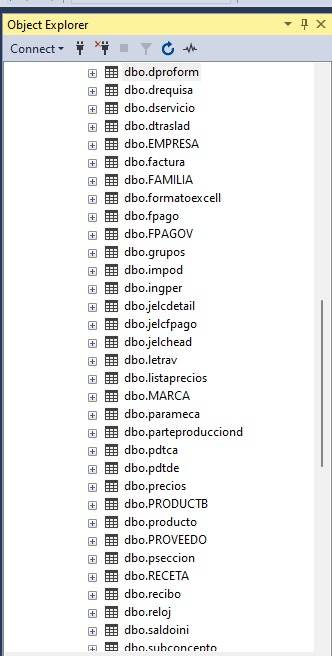
\includegraphics[width=0.5\textwidth]{3/figures/tablaSQL.jpg}
				\caption{Tablas de ventas}
				\textit{Fuente: Elaboración propia}
				\label{fig:tablasql}
			\end{center}	
		\end{figure}
		
		
		
		
		
		%\LaTeX{} is great at typesetting mathematics. Let $X_1, X_2, \ldots, X_n$ be a sequence of independent and identically distributed random variables with
		%\begin{equation}
		%	S_n = \frac{X_1 + X_2 + \cdots + X_n}{n}
		%	= \frac{1}{n}\sum_{i}^{n} X_i
		%	\label{eq1}
		%\end{equation}
		
		%La Ecuación \ref{eq1} denote their mean. Then as $n$ approaches infinity, the random variables $$\sqrt{n}(S_n - \mu)$$ converge in distribution to a normal $\mathcal{N}(0, \sigma^2)$.
		
		
		\section{Técnicas para el procesamiento y análisis de la información}
		Para entrar con más detalles a la metodología se describen los pasos a seguir.
		
		
		\subsection{Metodología de la implementación de la solución}
		El primer paso en el proceso KDD (Knowledge Discovery in Databases) consiste en la comprensión y selección de los datos disponibles, así como en la definición clara de los objetivos de la investigación desde la perspectiva del investigador. Este proceso se fundamenta en el conocimiento previo y adquirido durante el estudio. En el contexto del análisis de tendencias de ventas a lo largo del tiempo, este paso implica examinar minuciosamente aspectos como el monto de la transacción, la fecha y hora de compra, la cantidad adquirida, la categoría de producto (familia) y el producto específico.
		Además, resulta esencial definir con precisión los objetivos específicos de la investigación, tales como la identificación de patrones de comportamiento en las series temporales de ventas. Estos objetivos guían el análisis detallado y permiten enfocar la metodología hacia la detección de patrones útiles que faciliten la toma de decisiones y la optimización de la gestión de demanda en productos perecibles.
		
				
		\begin{figure}[H]
			\begin{center}
				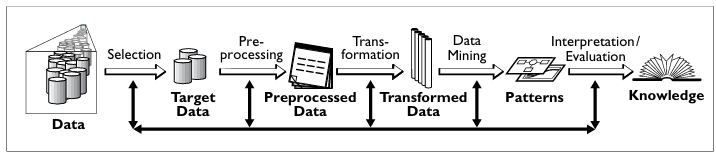
\includegraphics[width=0.9\textwidth]{2/figures/KDD.png}
				\caption{Metodología KDD}
				\textit{Fuente: Fayyad, U., Piatetsky-Shapiro, G.,  Smyth, P. (1996). The KDD process for extracting useful knowledge from volumes of data. Communications of the ACM, 39(11), 27-34.}
				\label{fig:KDD}
			\end{center}	
		\end{figure}
		
		\begin{table}[H]
			\centering
			\caption{Instrumentos de medida para recolección de datos}
			\begin{tabular}{|L{2.7cm}|L{2.5cm}|C{2cm}|C{3.5cm}|C{3.5cm}|}
				\hline 
				Técnica & Instrumento & Origen & Principales ventajas & Principales desventajas\\
				\hline \hline
				Datos de ventas históricas & Registro de ventas(2012-2026) & Registro de la empresa & Obtiene datos cuantitativos sobre las ventas históricas de productos & No proporciona informacion cualitativa sobre los patrones de la demanda  \\
				\hline
				Sistemas de punto de venta (POS) & Hardware POS & Registro en tiempo real de transacciones & Ofrece datos continuos y actualizados sobre las ventas & Dependencia de la confiabilidad del sistema \\
				\hline
				Datos de inventarios & Registro de inventarios & Registro de la empresa & Permite evaluar la relación entre la demanda y la gestión de inventarios Cuantitativamente & No proporciona información sobre factores externos\\
				\hline
%				Análisis de datos climaticos & Datos climáticos & Registros & Permite cuantificar como las condiciones climáticas influyen en la demanda & No considera factores anómalos climáticos\\
%				\hline
				
			\end{tabular}
			\newline
			\newline \textit{Fuente: Elaboración propia}
		\end{table}
		
		Esta comprensión inicial es fundamental para orientar las etapas siguientes de la metodología KDD y garantizar que el análisis de los datos sea relevante y eficaz. La selección de la base de datos adecuada y de las variables para el modelo de aprendizaje automático se realizará utilizando la base de datos proporcionada por la entidad en este caso de estudio.
		
		
		% \subsection{Comprensión del negocio}
		% En la fase inicial, se identificó el problema mediante la comprensión del contexto de la investigación. A partir de esta comprensión, se establecieron los objetivos y requisitos esperados para el proyecto. La siguiente tabla muestra la lista de actividades y tareas planificadas.
		
		% \begin{table}[H]
		% 	\centering
		% 	\caption{Actividades de la comprensión de negocio}
		% 	\begin{tabular}{L{3cm}|L{5cm}|L{5cm}}
				
		% 		Actvidades & Descripción & Tareas \\
		% 		\hline \hline
		% 		Definir problemas, objetivos e hipotesis. & Se definieron los problemas, objetivos, e hipótesis tanto generales como específicos de la investigación. &  
		% 		\begin{itemize}
		% 			\item Identificar la problemática del contexto.
		% 			\item Establecer los objetivos de la investigación.
		% 			\item Formular las hipótesis del estudio.
		% 		\end{itemize}
		% 		\\
		% 		\hline
		% 		Desarrollar la literatura de la investigación. & Se realizó una selección de antecedentes y estudios previos relacionados con la investigación. & 
		% 		\begin{itemize}
		% 			\item Buscar estudios relacionados al tema, la metodología y solución.
		% 		\end{itemize} \\
		% 		\hline	
		% 		Definir metodología de la investigación. & Se definió la metodología a implementarse en el estudio. & 
		% 		\begin{itemize}
		% 			\item Seleccionar la metodología a implementar en base a la investigación de antecedentes.
		% 		\end{itemize}
		% 		\\
		% 		\hline
				
		% 	\end{tabular}
		% 	\newline
		% 	\newline \textit{Fuente: Elaboración propia}
		% \end{table}
		
		
		% \textbf{Actividad 1: } Definir problemas, objetivos e hipótesis.\\
		% Esta actividad describe cómo se identificaron los problemas y se establecieron los objetivos e hipótesis, tanto generales como específicos, de la investigación, basándose en el análisis de la situación problemática actual.\\
		% \textbf{Entregable: } Problemas, objetivos e hipótesis.
		
		% \textbf{Actividad 2: } Desarrollar la literatura de la investigación.\\
		% Una vez definidos los objetivos, se llevó a cabo la búsqueda de fuentes, publicaciones, libros, artículos y material académico relacionado con el contexto, sus características y los métodos empleados para resolver problemas en ese entorno. Además, se desarrolló el marco teórico del estudio.\\
		% \textbf{Entregable: } Antecedentes académicos en la forma de objetivo, base de datos, metodología y resultados en el contexto de la investigación
		
		% \textbf{Actividad 3: } Definir la metodología de la investigación.\\
		% Después de obtener suficientes recursos intelectuales y revisar los trabajos previos necesarios para el desarrollo de la investigación, se analizaron detalladamente cada uno de los antecedentes y se compararon las metodologías implementadas por distintos autores. Al finalizar esta tarea, y con base en la literatura y los procesos más alineados con el presente estudio, se seleccionó la metodología KDD como la opción más adecuada.\\
		% \textbf{Entregable: } Metodología a implementar.
		
		
		\subsection{Comprensión de los datos}
		La investigación incluyó un proceso exhaustivo de exploración, análisis e interpretación de la información recopilada, con el objetivo de identificar patrones, tendencias y relaciones significativas. Este paso es fundamental para garantizar que los datos sean relevantes, precisos y útiles para responder a las preguntas de investigación y alcanzar los objetivos del estudio. El conjunto de datos utilizado abarca 7,340,659 registros de ventas, organizados por familia de productos, correspondientes a los años 2012 al 2026. 
		% Para mayor claridad, se elaboró una tabla que presenta las actividades y tareas realizadas. \ref{tab:compredatos}
		
		% \begin{table}[H]
		% 	\centering
		% 	\caption{Actividades de la Comprensión de los datos}
		% 	\begin{tabular}{L{3cm}|L{5cm}|L{5cm}}
				
		% 		Actvidades & Descripción & Tareas \\
		% 		\hline \hline
		% 		Selección de la base de datos & Base de datos que contenga variables que aporten al modelo y representen significancia al pronóstico & 
		% 		\begin{itemize}
		% 			\item Construir los query en SQL para seleccionar las variables representativas para la ivestigación.
		% 			\item Agrupar las variables por familias para preparar el análisis.
		% 		\end{itemize} \\
		% 		\hline
		% 		Analisis bivariado y univariado & Análisis del comportamiento de las variables y en la descripción y resumen de una sola variable a la vez para entender y representar las características básicas & 
		% 		\begin{itemize}
		% 			\item Construir los scrips en python para analizar variables y pares de variables. 
		% 			\item Entender las características de cada variable.
		% 		\end{itemize} \\
		% 		\hline
		% 		%		Análisis estadístico & Analisis estadístico para interpretar y presentar datos cuantitativos para descubrir patrones, tendencias y relaciones significativas & 
		% 		%		\begin{itemize}
		% 			%			\item Analizar el comportamiento estadístico de cada variable cuantitativa.
		% 			%			
		% 			%		\end{itemize} \\
		% 		%		\hline
		% 	\end{tabular}
		% 	\label{tab:compredatos}
		% 	\newline
		% 	\newline \textit{Fuente: Elaboración propia}
		% \end{table}
		
		
		% \textbf{Actividad 1: }Selección de la base de datos. \\
		% La selección de los datos en SQL implicó escoger una base de datos con variables específicas del negocio dentro de un sistema de gestión de bases de datos (DBMS).
		
		% \begin{figure}[H]
		% 	\begin{center}
		% 		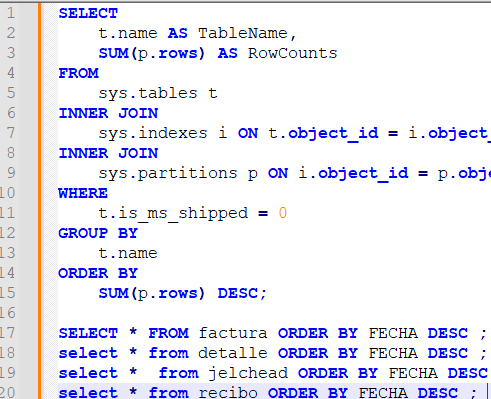
\includegraphics[width=0.6\textwidth]{3/figures/select_tablas.png}
		% 		\caption{Selección de tablas SQL}
		% 		\textit{Fuente: Elaboración propia}
		% 		\label{fig:consultaSQL}
		% 	\end{center}	
		% \end{figure}
		
		\begin{figure}[H]
			\begin{center}
				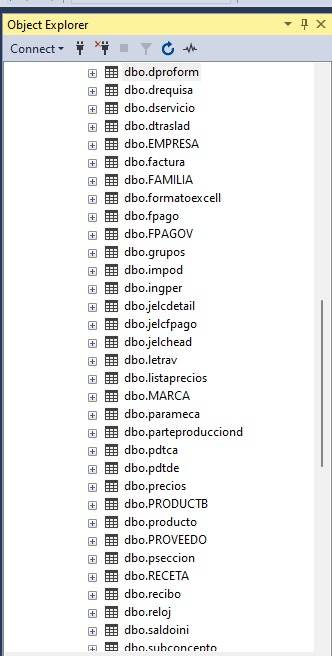
\includegraphics[width=0.6\textwidth]{3/figures/tablaSQL.jpg}
				\caption{Tablas de ventas}
				\textit{Fuente: Elaboración propia}
				\label{fig:tablaSQL}
			\end{center}	
		\end{figure}
		
		
		% \textbf{Entregable: }  Tablas de ventas 
		
		% \textbf{Actividad 2: }Analisis bivariado y univariado. \\
		Se emplearon análisis univariado y bivariado para examinar y comprender los datos. El análisis univariado se centró en describir y resumir una sola variable a la vez, utilizando estadísticas como la media, mediana, moda y varianza, además de visualizaciones como histogramas para revelar la distribución y características específicas de esa variable. Por otro lado, el análisis bivariado se enfocó en explorar la relación entre dos variables, empleando técnicas como tablas de correlación y regresión para identificar patrones, asociaciones y posibles causalidades entre las variables.
	
		\begin{figure}[H]
    \centering
    
    \begin{subfigure}{0.45\textwidth}
        \centering
        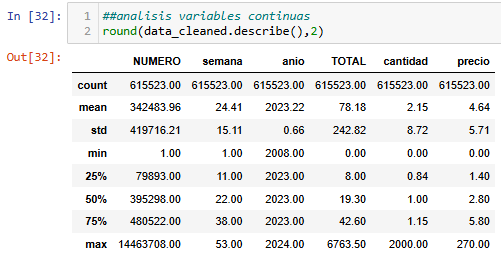
\includegraphics[width=\linewidth]{3/figures/descrip_var.png}
        \caption{Descripción cuantitativa}
        \label{fig:descrip_var}
    \end{subfigure}
    \hfill
    \begin{subfigure}{0.45\textwidth}
        \centering
        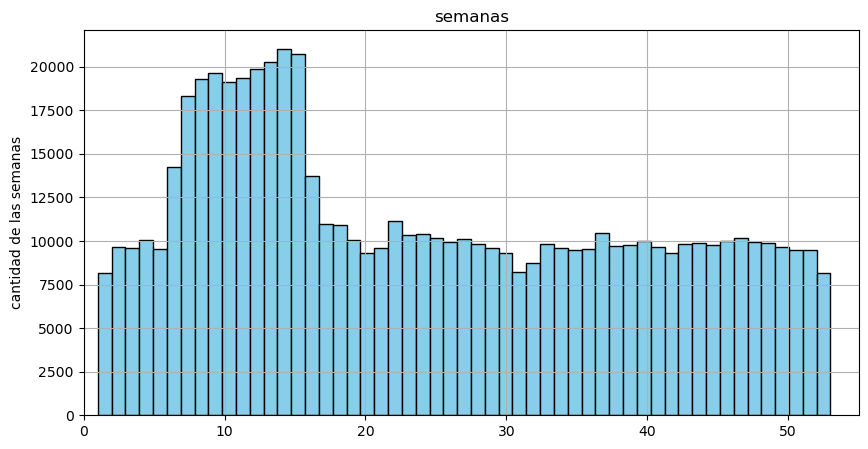
\includegraphics[width=\linewidth]{3/figures/cant_sem.png}
        \caption{Cuantificación de semanas}
        \label{fig:cant_sem}
    \end{subfigure}

    \vspace{0.5cm}

    \begin{subfigure}{0.45\textwidth}
        \centering
        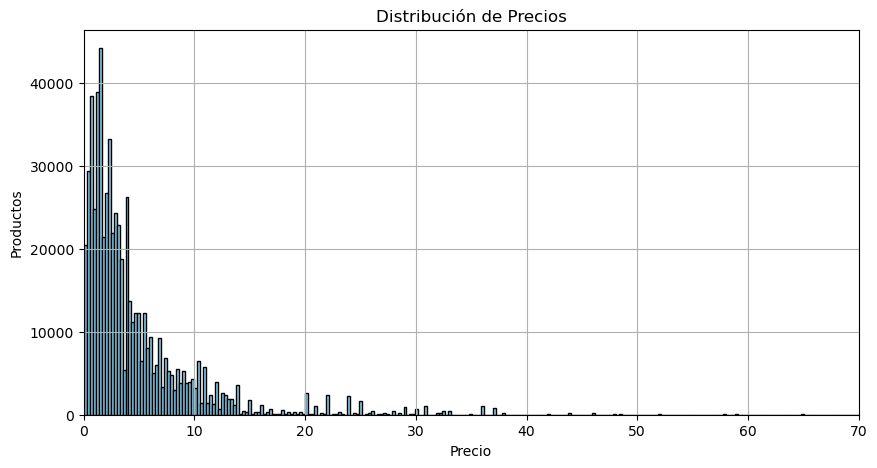
\includegraphics[width=\linewidth]{3/figures/distr_precios.png}
        \caption{Distribución de precio}
        \label{fig:distr_precios}
    \end{subfigure}
    \hfill
    \begin{subfigure}{0.45\textwidth}
        \centering
        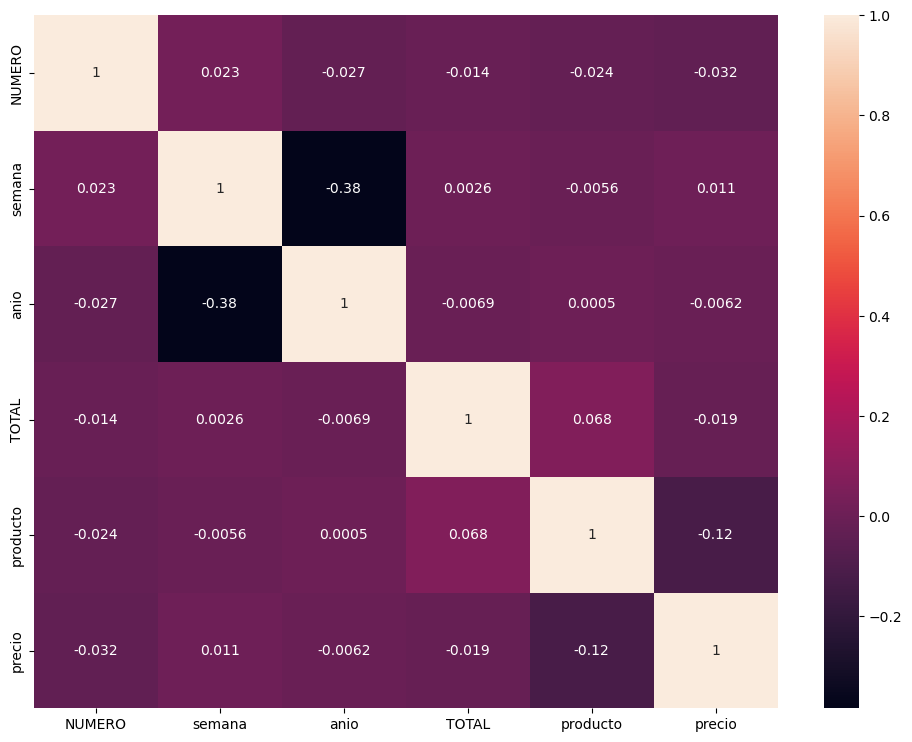
\includegraphics[width=\linewidth]{3/figures/corr_var.png}
        \caption{Correlación de variables}
        \label{fig:corr_var}
    \end{subfigure}

    \caption{Análisis exploratorio de variables}
    \textit{Fuente: Elaboración propia}
    \label{fig:analisis_exploratorio}
\end{figure}
	
		% \begin{figure}[H]
		% 	\begin{center}
		% 		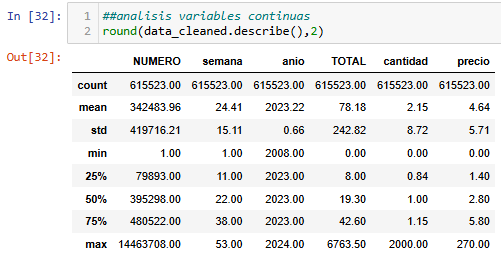
\includegraphics[width=0.6\textwidth]{3/figures/descrip_var.png}
		% 		\caption{Descripción cuantitativa}
		% 		\textit{Fuente: Elaboración propia}
		% 		\label{fig:descrip_var}
		% 	\end{center}	
		% \end{figure}
		
		% \begin{figure}[H]
		% 	\begin{center}
		% 		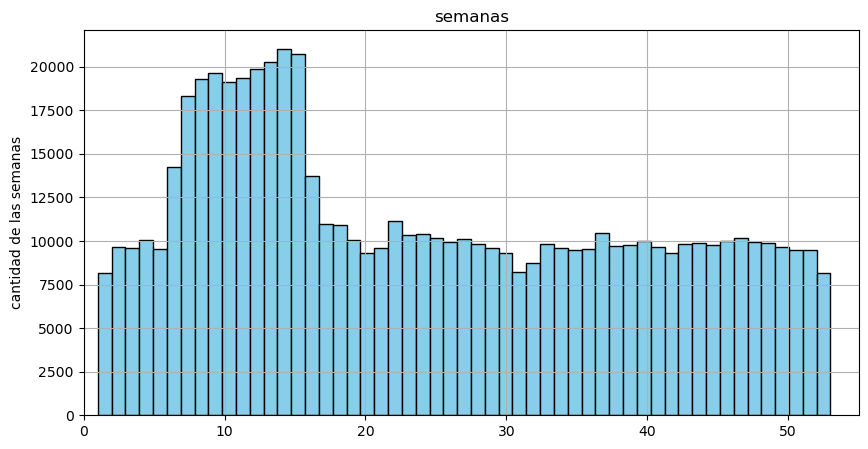
\includegraphics[width=0.6\textwidth]{3/figures/cant_sem.png}
		% 		\caption{Cuantificación de semanas}
		% 		\textit{Fuente: Elaboración propia}
		% 		\label{fig:cant_sem}
		% 	\end{center}	
		% \end{figure}
		
		% \begin{figure}[H]
		% 	\begin{center}
		% 		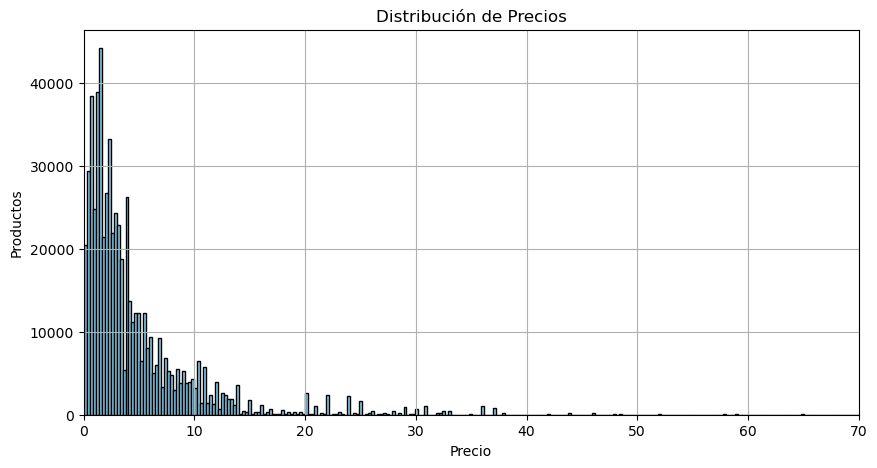
\includegraphics[width=0.6\textwidth]{3/figures/distr_precios.png}
		% 		\caption{Distribución de precio}
		% 		\textit{Fuente: Elaboración propia}
		% 		\label{fig:distr_precios}
		% 	\end{center}	
		% \end{figure}
		
		% \begin{figure}[H]
		% 	\begin{center}
		% 		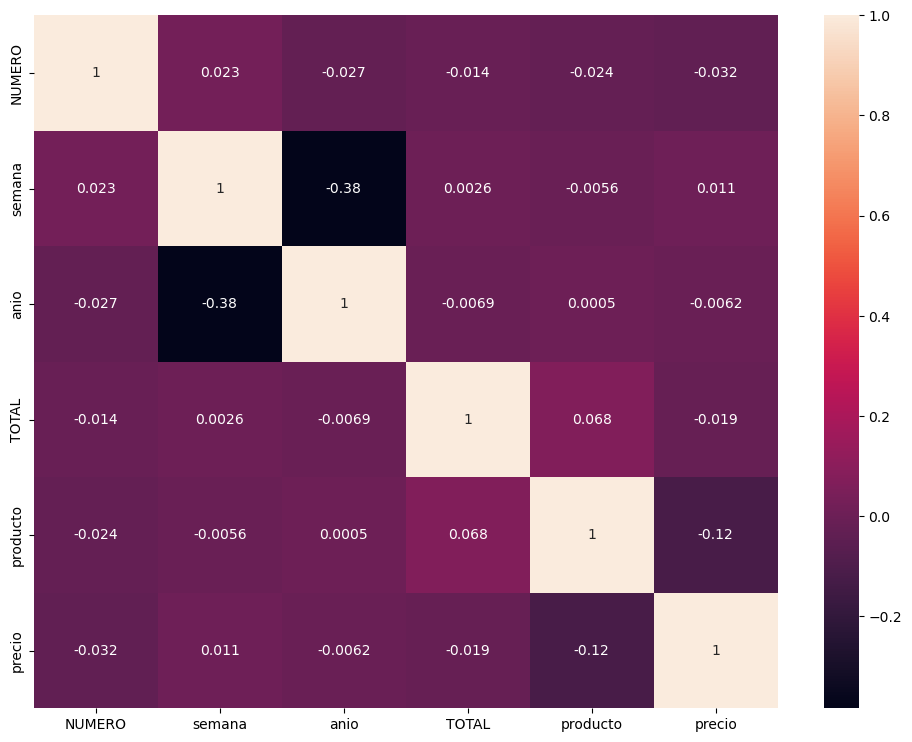
\includegraphics[width=0.6\textwidth]{3/figures/corr_var.png}
		% 		\caption{Correlación de variables}
		% 		\textit{Fuente: Elaboración propia}
		% 		\label{fig:corr_var}
		% 	\end{center}	
		% \end{figure}
		
		El mapa de calor muestra la correlación entre varias variables, como semana, año, total, producto, y precio. En general, las correlaciones son débiles, con solo una correlación negativa moderada entre semana y año (-0.38). Esto sugiere que no hay relaciones lineales fuertes entre las variables, lo cual indica que cada una aporta información única al conjunto de datos. Este análisis preliminar sugiere que no es necesario eliminar ninguna columna por redundancia, ya que las correlaciones no son suficientemente altas.
		
		% \textbf{Entregable: } Análisis estadístico de variables
		
		\subsection{Pre-Procesamiento}
		% Una vez integrada la información en la base de datos, se desarrolló la etapa de preprocesamiento de datos, cuyo objetivo principal fue garantizar la calidad, consistencia y confiabilidad de la información antes de realizar el análisis exploratorio y el entrenamiento de los modelos predictivos.

En esta fase se efectuó, en primer lugar, la normalización de los nombres de las variables, con la finalidad de mantener una estructura homogénea dentro del conjunto de datos y evitar inconsistencias durante el procesamiento. Posteriormente, las variables de tipo temporal fueron convertidas a un formato de fecha estándar, permitiendo ordenar cronológicamente los registros y facilitar el análisis de series temporales.

Asimismo, las variables numéricas relacionadas con las ventas fueron transformadas al tipo de dato correspondiente para asegurar su correcta interpretación por parte de los algoritmos de análisis. Durante este proceso también se identificaron y eliminaron registros incompletos, inconsistentes o con valores inválidos, especialmente aquellos asociados a fechas o montos de venta no reconocidos.

Después de la limpieza inicial, los datos fueron ordenados secuencialmente según la variable temporal. Este procedimiento resulta fundamental en problemas de predicción temporal, debido a que los modelos requieren preservar la relación cronológica entre observaciones históricas y futuras.

Posteriormente, se realizó la segmentación de la información según criterios específicos de análisis, tales como la sede y la familia de productos. Esta segmentación permitió trabajar con subconjuntos de datos más homogéneos y representativos, contribuyendo a mejorar la precisión y pertinencia de los modelos predictivos.

Finalmente, el preprocesamiento permitió obtener un conjunto de datos estructurado, consistente y preparado para las etapas posteriores de análisis exploratorio, entrenamiento y evaluación de modelos de predicción.
		
		
		% \subsection{Procesamiento}
		% El segundo paso en la metodología KDD se centra en la preparación de los datos de transacciones de ventas de manera diaria. Este proceso implica realizar operaciones básicas de limpieza y depuración, eliminando ruido y valores atípicos que puedan afectar la calidad y precisión de los resultados. Además, se recopila información relevante para entender y modelar el ruido presente en los datos, lo que facilita una interpretación más clara de los patrones y tendencias. Se implementan también estrategias para gestionar campos de datos que carecen de información cronológica, asegurando así la coherencia y cohesión de los datos para un análisis efectivo.
		
		% \subsection{Transformación}
		% En el tercer paso de la metodología KDD, se realiza la transformación de datos para adecuarlos al análisis, centrándose en agrupar los productos por familias. Esta fase implica identificar características que representen eficazmente los datos y que se ajusten a los objetivos específicos de la tarea de análisis. Según estos objetivos, se seleccionan las características más relevantes para proporcionar información significativa sobre las ventas. Además, se aplican técnicas para reducir la complejidad de los datos o encontrar representaciones más concisas y manejables. Este proceso es fundamental para simplificar la estructura de los datos y facilitar un análisis más eficiente y efectivo.
		
		%\subsection{Modelado}
		%En el cuarto paso de la metodología KDD, se profundiza en la minería de datos para predecir las ventas. Aquí, la selección adecuada de algoritmos es crucial para descubrir patrones significativos en los datos, considerando su naturaleza, los objetivos de la predicción y la complejidad del análisis requerido. Se ajustan los parámetros de los algoritmos para mejorar el rendimiento del modelo predictivo y se evalúa la idoneidad de cada método para asegurar predicciones precisas sobre las ventas.
		%
		%\subsection{Evaluación}
		%En el cuarto paso de la metodología KDD, se aborda la interpretación de patrones y la selección de algoritmos para predecir las ventas semanales, segmentadas por familias como verduras, frutas, carnes, entre otros. Es crucial evaluar la efectividad de los algoritmos en la detección de patrones significativos en los datos y estar preparado para ajustar el análisis retrocediendo a pasos anteriores si es necesario.
		%La capacidad de visualizar los patrones extraídos es esencial para comprender la serie temporal de las ventas, lo que facilita la identificación de las familias con mayor porcentaje de venta y la estimación de presupuestos semanales basados en la demanda. Durante este proceso, se eliminan patrones redundantes o irrelevantes para centrarse en aquellos más pertinentes para el análisis de ventas. Finalmente, estos patrones se convierten en términos comprensibles para los usuarios, facilitando la toma de decisiones informadas y la implementación de estrategias efectivas de compra de mercadería.
		
		\subsection{Modelamiento}
		Al concluir la etapa del preprocesamiento, las variables pudieron ser utilizadas para los modelos de cada modalidad, que fueron diseñados siguiendo las actividades de la Tabla \ref{tab:act_model}
		
		\begin{table}[H]
			\centering
			\caption{Actividades de fase modelamiento}
			\begin{tabular}{L{3cm}|L{5cm}|L{5cm}}
				
				Actvidades & Descripción & Tareas \\
				\hline \hline
				Desarrollar modelos predictivos para data estructurada. & Implementación de un mínimo de 8 modelos de forecasting para entrenarlos y seleccionar el mejor para la data.  &  Escoger los modelos para entrenarlos y ver cual es el mejor modelo para realizar los pronósticos de ventas.
				
				\\
				\hline
				Seleccionar las métricas para la evaluación del modelo. & Implementación las métricas para poder evaluar a los modelos implementados. & Escoger las métricas que definirán cual modelo será mejor para realizar los pronósticos de venta (R2, MSE, RMSE y MAPE).
				\\
				\hline	
				
			\end{tabular}
			\newline
			\newline \textit{Fuente: Elaboración propia}
			\label{tab:act_model}
		\end{table}
		
		\textbf{Actividad 1: } Desarrollar modelos predictivos para data estructurada.\\
		En esta actividad, se diseñó la arquitectura que se utilizó para los datos estructurados. Para ello, se llevó a cabo un benchmarking sobre los modelos a utilizar:
		\begin{itemize}
			\item \textbf{ARIMA: } ARIMA es un modelo estadístico utilizado para analizar y predecir series temporales. Combina la parte autoregresiva (AR), que utiliza las observaciones pasadas para predecir valores futuros, con la parte de media móvil integrada (IMA), que maneja la variabilidad y tendencia de los datos.
			\item \textbf{LSTM: } LSTM es un tipo de red neuronal recurrente (RNN) diseñada para modelar secuencias temporales y dependencias a largo plazo. Es capaz de aprender dependencias temporales en los datos y es especialmente efectiva en problemas donde las relaciones entre eventos en el tiempo son importantes.
			\item \textbf{LINEAR REGRESSION: } La regresión lineal es un modelo estadístico que examina la relación lineal entre una variable dependiente y una o más variables independientes. El objetivo es encontrar la línea (o plano en casos de múltiples variables) que mejor se ajuste a los datos, minimizando la suma de los errores cuadráticos.
			\item \textbf{XGBOOST: } XGBoost es una implementación optimizada del algoritmo de gradient boosting, que se utiliza ampliamente en problemas de aprendizaje supervisado, tanto para clasificación como para regresión. Utiliza árboles de decisión como modelos base y se enfoca en mejorar el rendimiento a través de técnicas como la regularización y el manejo eficiente de conjuntos de datos grandes.
			\item \textbf{SVR: } SVR es una variante de las máquinas de vectores de soporte (SVM) adaptada para problemas de regresión. A diferencia de los métodos de regresión lineal, SVR utiliza vectores de soporte en un espacio de alta dimensión para predecir valores continuos, buscando la función que mejor se ajuste a los datos mientras mantiene un margen de error aceptable.
			\item \textbf{RANDOM FOREST: } Random Forest es un conjunto de árboles de decisión, donde cada árbol es construido de manera independiente y con muestras de datos aleatorias. La predicción final se obtiene por votación o promediando las predicciones individuales de los árboles, lo que mejora la precisión y reduce el sobreajuste.
			\item \textbf{DECISION TREE: } Un árbol de decisión es una estructura de modelo de aprendizaje automático que divide un conjunto de datos en subconjuntos más pequeños basados en características específicas de las variables predictoras. Cada nodo representa una característica y cada hoja representa un resultado o decisión.
			\item \textbf{PROPHET: } Prophet es un modelo desarrollado por Facebook para realizar pronósticos de series temporales. Es especialmente útil cuando se cuenta con datos estacionales, festivos o fluctuaciones regulares, y permite manejar datos con puntos faltantes o valores atípicos. Es fácil de usar y flexible para ajustar tendencias y patrones estacionales.
			\item \textbf{GRADIENT BOOSTING: } Gradient Boosting es un algoritmo de aprendizaje supervisado que construye modelos de forma secuencial, donde cada nuevo modelo corrige los errores del anterior. Utiliza árboles de decisión como modelos base y optimiza una función de pérdida mediante el descenso de gradiente, logrando alta precisión en tareas de regresión y clasificación.

\item \textbf{KNN (K-Nearest Neighbors): } KNN es un algoritmo de aprendizaje basado en instancias que realiza predicciones basándose en los datos más cercanos en el espacio de características. Para regresión, el valor predicho se obtiene como el promedio de los valores de sus vecinos más cercanos, lo que lo hace simple pero efectivo en ciertos contextos.

\item \textbf{HOLT-WINTERS: } Holt-Winters es un método de suavizamiento exponencial utilizado para series temporales que presentan tendencia y estacionalidad. Este modelo combina componentes de nivel, tendencia y estacionalidad para realizar predicciones más precisas en datos con patrones periódicos.

\item \textbf{NAIVE: } El modelo Naive es un enfoque simple de pronóstico en series temporales que asume que el valor futuro será igual al último valor observado. A pesar de su simplicidad, se utiliza como modelo base para comparar el rendimiento de modelos más complejos.

\item \textbf{SARIMA: } SARIMA (Seasonal ARIMA) es una extensión del modelo ARIMA que incorpora componentes estacionales. Permite modelar tanto patrones no estacionales como estacionales en series temporales, siendo útil cuando los datos presentan ciclos repetitivos a lo largo del tiempo.
		\end{itemize}
		
		Con base en la revisión de estudios previos, se observó que los modelos LSTM, Regresión Lineal y Árbol de Decisión ofrecieron los mejores resultados en experimentos similares. Dado que el objetivo de la investigación era implementar un modelo de regresión, se decidió utilizar Regresion Lineal para el análisis de los datos estructurados.
		
		\textbf{Diseño de la Arquitectura Regresion Lineal Multiple}
		
		La ecuación general de la regresión lineal múltiple se define como:  
		
		\begin{equation}
		Y = \beta_0 + \beta_1 X_1 + \beta_2 X_2 + \cdots + \beta_n X_n + \epsilon
		\end{equation}
		
		Donde:  
		\begin{itemize}
			\item \( Y \): Variable dependiente o respuesta.
			\item \( X_1, X_2, \dots, X_n \): Variables independientes o explicativas.
			\item \( \beta_0 \): Intercepto o término constante.
			\item \( \beta_1, \beta_2, \dots, \beta_n \): Coeficientes de las variables independientes, que representan su contribución al valor de \( Y \).
			\item \( \epsilon \): Error residual, que captura las desviaciones no explicadas por el modelo.
		\end{itemize}
		
		El objetivo es estimar los coeficientes \( \beta_0, \beta_1, \dots, \beta_n \) que minimicen la suma de los errores al cuadrado (Método de Mínimos Cuadrados Ordinarios):  
		
		\begin{equation}
		\text{Minimizar: } \sum_{i=1}^m \left( Y_i - \hat{Y}_i \right)^2
		\end{equation}
		
		Donde \( \hat{Y}_i \) es el valor predicho para la \( i \)-ésima observación.  
		
%		Para diseñar la arquitectura del modelo LSTM, se evaluaron diversas metodologías y estrategias. Finalmente, se seleccionaron las siguientes 12 pautas fundamentales para su implementación:
%		
%		\begin{enumerate}
%			\item Comenzar con al menos 2 capas LSTM para capturar dependencias a largo plazo en los datos secuenciales. 
%			\item El número de unidades en las capas LSTM puede variar dependiendo de la complejidad del problema y la cantidad de datos disponibles. Puedes experimentar con diferentes números de unidades, como 50, 100 o más.
%			\item Utilizar una capa densa con una unidad para la predicción de ventas, con función de activación lineal.
%			\item Utilizar la función de activación 'tanh' o 'sigmoid' para las capas LSTM para introducir no linealidades en el modelo.
%			\item Aplicar dropout después de cada capa LSTM para mejorar la generalización del modelo, con una tasa recomendada del 0.2 o ajustada según experimentación.
%			\item Escalar los datos secuenciales utilizando métodos como MinMaxScaler o StandardScaler según la naturaleza de los datos y su distribución.
%			\item Utilizar métricas como el error cuadrático medio (MSE) o el error absoluto medio (MAE) para evaluar el rendimiento del modelo de predicción.
%			\item Comenzar con un número adecuado de épocas, por ejemplo, 20 épocas, y ajustar según la mejora en la precisión y la reducción de la pérdida. Aumentar gradualmente hasta 100 épocas si es necesario para mejorar el rendimiento del modelo LSTM.
%			\item Utilizar la función 'train\_test\_split' para dividir los datos en conjuntos de entrenamiento y prueba. Asegúrate de que los datos estén divididos de manera que se mantenga la secuencia temporal, es decir, no barajar los datos.
%			\item No aplica directamente para predicción de ventas, pero asegúrate de que tus datos están correctamente representados y no tienen sesgos significativos que puedan afectar la predicción.
%			\item Utilizar el optimizador 'Adam' con sus configuraciones por defecto para el aprendizaje de los pesos de la red neuronal LSTM.
%			\item Aplicar técnicas de regularización como L2 para evitar el sobreajuste del modelo 
%			
%		\end{enumerate}
		
		\textbf{Entregable: } Modelo Regresion Lineal para el pronostico de ventas.
		
		\textbf{Actividad 2: } Seleccionar las métricas para la evaluación del modelo
		En esta actividad, se llevó a cabo una investigación basada en el estado del arte para identificar las métricas ma´s utilizadas en investigaciones previas. Se encontró que las métricas más frecuentemente empleadas fueron las siguientes:
		
		
		\begin{itemize}
			\item \textbf{RMSE: } Calcula la raíz cuadrada de la media de los cuadrados de los errores entre las predicciones de un modelo y los valores reales. Es útil para medir el nivel de error promedio de las predicciones en la misma unidad que los datos originales.
			\item \textbf{MSE: } Calcula el promedio de los cuadrados de los errores entre las predicciones de un modelo y los valores reales. Proporciona una medida de la varianza de los errores, penalizando más fuertemente los errores grandes.
			\item \textbf{MAPE: } Calcula el promedio del porcentaje absoluto de los errores entre las predicciones de un modelo y los valores reales. Es útil para evaluar la precisión relativa de un modelo, especialmente en situaciones donde se desea conocer el error porcentual promedio. 
		\item \textbf{R2: } Calcula el coeficiente de determinación, que mide la proporción de la variabilidad en los datos que es explicada por el modelo. Un valor de R2 cercano a 1 indica un buen ajuste del modelo a los datos, mientras que un valor cercano a 0 indica un ajuste pobre.
		\end{itemize}
		
		De acuerdo a la anterior lista, estas métricas ayudarán a:
		
		\begin{itemize}
			\item Evaluar la precisión y el rendimiento de modelos predictivos en comparación con los valores reales.
			\item Cuantificar el nivel de error y la discrepancia entre las predicciones del modelo y los datos observados.
			\item Optimizar y ajustar los parámetros del modelo para minimizar el error y mejorar la precisión de las predicciones.
		\end{itemize}
		
% 		Estas métricas proporcionan una base sólida para la evaluación rigurosa de modelos predictivos en diversas aplicaciones, facilitando la toma de decisiones informadas y la mejora continua del rendimiento del modelo.\\
		
% 		Las métricas señaladas se calculan de la siguiente manera: \\
		
% 		\textbf{RMSE (Root Mean Square Error)}\\
		
% 		\textbf{Calcular los errores individuales: } Para cada predicción \(\hat{y}_i\) y su valor real \(y_i\), calcula el error cuadrático.
		
% 		\begin{equation} 
% 			\text{Error}_i = (\hat{y}_i - y_i)^2
% 		\end{equation}
		
% 		\textbf{Calcular el promedio de los errores cuadráticos: } Luego, calcula el promedio de estos errores cuadráticos sobre todos los puntos de datos.
		
% 		\begin{equation} 
% 			\text{MSE} = \frac{1}{n} \sum_{i=1}^{n} (\hat{y}_i - y_i)^2
% 		\end{equation}
		
% 		\textbf{Calcular la raíz cuadrada del MSE: } Finalmente, obtén el RMSE tomando la raíz cuadrada del MSE.
% 		\begin{equation}
% 			\text{RMSE} = \sqrt{\text{MSE}}
% 		\end{equation}
		
% 		\textbf{MSE (Mean Squared Error)}\\
% 		\textbf{Calcular los errores individuales: } Para cada predicción \(\hat{y}_i\) y su valor real \(y_i\), calcula el error cuadrático como en el paso 1 del RMSE:
% 		\begin{equation}
% 			\text{Error}_i = (\hat{y}_i - y_i)^2
% 		\end{equation}
		
% 		\textbf{Calcular el promedio de los errores cuadráticos: } Luego, calcula el promedio de estos errores cuadráticos sobre todos los puntos de datos. 
		
% 		\begin{equation}
% 			\text{MSE} = \frac{1}{n} \sum_{i=1}^{n} (\hat{y}_i - y_i)^2
% 		\end{equation}
		
% 		\textbf{MAPE (Mean Absolute Percentage Error)}\\
% 		\textbf{Calcular los errores porcentuales individuales: } Para cada predicción \(\hat{y}_i\) y su valor real \(y_i\), calcula el error porcentual absoluto.
		
% 		\begin{equation}
% 			Error_i = \left( \frac{y_i - \hat{y}_i}{y_i} \right) \times 100
% 		\end{equation}
		
% 		\textbf{Calcular el promedio de los errores porcentuales: } Luego, calcula el promedio de estos errores porcentuales sobre todos los puntos de datos.
% 		%%%%%AGREGAR R2
% 		\begin{equation}
% 			\text{MAPE} = \frac{1}{n} \sum_{i=1}^n \left( \frac{|y_i - \hat{y}_i|}{y_i} \right) \times 100
% 		\end{equation}
		
% 		\textbf{Entregable: } Modelo LSTM entrenado con sus respectivas métricas.
		
% 		%%%%%%%%%%%%%%%%%%%
% 		\textbf{MAE (Mean Absolute Error): } El MAE es una métrica utilizada para evaluar la precisión de modelos de regresión. Mide el promedio de los errores absolutos entre los valores reales y los valores predichos, sin considerar la dirección del error. Es fácil de interpretar, ya que expresa el error promedio en las mismas unidades que la variable objetivo.
% 		\textbf{Fórmula del MAE: }
% 		\[
% 		MAE = \frac{1}{n} \sum_{i=1}^{n} \left| y_i - \hat{y}_i \right|
% \]
% \textbf{R2 (Coeficiente de Determinación): } El R2 es una métrica que mide la proporción de la variabilidad en los datos que es explicada por el modelo de regresión. Un valor de R2 cercano a 1 indica que el modelo explica la mayor parte de la variabilidad, mientras que un valor cercano a 0 indica que el modelo no explica bien los datos.
% \textbf{Fórmula del R2: }
% \[
% R^2 = 1 - \frac{\sum_{i=1}^{n} (y_i - \hat{y}_i)^2}{\sum_{i=1}^{n} (y_i - \bar{y})^2}
% \]
% Donde \( \bar{y} \) es la media de los valores reales \( y_i \).

		\subsection{Evaluación}
		Esta fase comprende la evaluación de los modelos desarrollados en la investigación a través de las métricas de regresión seleccionadas y explicadas en la sección 3.3.6. En la Tabla \ref{tab:act_eva} se indican las actividades y tareas seguidas para esta etapa.
		
		\begin{table}[H]
			\centering
			\caption{Actividades de fase evaluación}
			\begin{tabular}{L{3cm}|L{5cm}|L{5cm}}
				
				Actvidades & Descripción & Tareas \\
				\hline \hline
				Evaluar el modelo predictivo & Evaluación del desempeño del modelo LSTM   & Ejecutar experimentos para definir hiperparámetros.		
				\\
				\hline
				Interpretar las métricas obtenidas & Observar los resultados de las métricas obtenidas permite inferir si el modelo puede ser un predictor confiable para los pronósticos. & Interpretar los resultados obtenidos de las métricas permite extraer conclusiones fundamentales sobre el rendimiento del modelo.
				\\
				\hline		
			\end{tabular}
			\newline
			\newline \textit{Fuente: Elaboración propia}
			\label{tab:act_eva}
		\end{table}
		
		\textbf{Actividad 1:} Evaluar el modelo predictivo.\\
		En esta actividad, se procedió inicialmente con el entrenamiento de todos los modelos utilizando datos recopilados durante aproximadamente 3 años, que incluyen las ventas semanales de la familia con la que se cuenta con mayor cantidad de datos históricos. Este proceso de entrenamiento fue fundamental para ajustar los modelos y capturar patrones y tendencias significativas basadas en un conjunto de datos robusto y representativo.
		Para optimizar el rendimiento de los modelos, se llevaron a cabo entre 3 y 5 experimentos por cada diseño de modelo, explorando diversas combinaciones y ajustes de hiperparámetros en cada iteración. Esta estrategia sistemática permitió evaluar cómo diferentes configuraciones afectan el rendimiento del modelo en términos de métricas críticas como precisión, error y capacidad de generalización.
		Los experimentos no solo se centraron en la optimización de hiperparámetros, sino también en la selección de técnicas de preprocesamiento de datos y ajustes de arquitectura del modelo. Cada iteración fue diseñada para obtener insights valiosos sobre qué configuraciones maximizan la capacidad del modelo para realizar pronósticos precisos y confiables de las ventas semanales.
		Este enfoque riguroso y metódico no solo aseguró la mejora continua del rendimiento predictivo, sino que también proporcionó una base sólida para la toma de decisiones informadas sobre la implementación y refinamiento del modelo finalmente seleccionado.\\
		
		\textbf{Entregable: } Modelo Regresión Lineal Entrenado y Ajustado.
		
		\textbf{Actividad 2: } Interpretar las métricas obtenidas.\\
		En esta actividad, se procedió inicialmente a realizar un análisis exhaustivo de las métricas obtenidas del modelo Regresion Lineal entrenado y ajustado. Estas métricas fueron meticulosamente calculadas para evaluar el desempeño del modelo en la predicción precisa de las ventas semanales, utilizando datos históricos recopilados durante aproximadamente 5 años.\\
		Durante el análisis, se focalizó en métricas fundamentales como el RMSE (Root Mean Square Error), MSE (Mean Squared Error) y MAPE (Mean Absolute Percentage Error). Estas métricas proporcionaron una evaluación cuantitativa del nivel de precisión y error del modelo en comparación con las ventas reales observadas en el período de entrenamiento.\\
		El estudio detallado de estas métricas permitió extraer conclusiones significativas sobre la capacidad del modelo para capturar variaciones y patrones en las ventas semanales. Además, facilitó la identificación de posibles áreas de mejora en términos de ajustes adicionales de hiperparámetros o refinamientos en la arquitectura del modelo Regresión Lineal.
		Este análisis crítico y sistemático es esencial para tomar decisiones informadas sobre la implementación y el desarrollo continuo del modelo Regresión Lineal en aplicaciones futuras de pronóstico de ventas. Asimismo, asegura un mejor rendimiento predictivo y una mayor precisión en la proyección de tendencias comerciales, beneficiando así la toma de decisiones estratégicas en el contexto empresarial.\\
		
		\textbf{Entregable: } Resultados de las métricas  MSE, RMSE, MAPE.
		
		\subsection{Despliegue}
		En la última fase de la metodología seguida, se implementó el modelo propuesto después de completar su entrenamiento y evaluación correspondiente. Esta etapa final fue crucial para poner a prueba la capacidad predictiva del modelo en un entorno operativo real. Las actividades detalladas realizadas durante esta fase se describen en la Tabla \ref{tab:fase_despl}, proporcionando una visión completa de los pasos ejecutados para asegurar la integración efectiva del modelo en la aplicación práctica.
		
		\begin{table}[H]
			\centering
			\caption{Actividades de fase Despliegue}
			\begin{tabular}{L{3cm}|L{5cm}|L{5cm}}
				
				Actvidades & Descripción & Tareas \\
				\hline \hline
				Diseñar prototipo de sistemas con modelo propuesto. & Diseño del prototipo del sistema que integrará la captura de datos con el modelo propuesto para predecir las ventas. &  
				\begin{itemize}
					\item Diseñar una estructura de prototipo de sistema conformado por captura de datos y modelo propuesto.
					\item Cargar complementos del modelo.
				\end{itemize}
				\\
				\hline
				Ejecutar el prototipo y integrarlo con el modelo desarrollado. & Ejecución del sistema prototipo en tiempo real con proyectos de tecnología de campañas vigentes. &
				\begin{itemize}
					\item Ejecutar prototipo con dirección web de proyecto consultado.
					\item Clasificar el estado de financiamiento a partir del resultado predicho.
				\end{itemize}
				\\
				\hline		
			\end{tabular}	
			\newline
			\newline \textit{Fuente: Elaboración propia}
			\label{tab:fase_despl}
		\end{table}
		
		Después de analizar el rendimiento de cada modelo, tanto individualmente como el modelo final, se compararon los resultados con los antecedentes disponibles. Luego, se llevó a cabo una prueba piloto donde se ejecutó el modelo ensamblado entrenado, se obtuvieron sus características y se realizaron predicciones tanto del presupuesto para cada familia de productos como de la cantidad de productos necesarios para realizar un pedido.
		
		\textbf{Actividad 1: } Diseñar prototipo de sistema con modelo propuesto\\
		En esta actividad, se diseñó el prototipo del sistema que integra el modelo propuesto para optimizar la gestión de inventarios y mejorar la precisión en las proyecciones de demanda. El sistema fue concebido para utilizar datos históricos y variables clave, permitiendo una planificación más eficiente de las operaciones y una mejor adaptación a las fluctuaciones del mercado.\\
		\textbf{Entregable: }Arquitectura del prototipo del sistema integrado.
		
		\textbf{Actividad 2: } Ejecutar prototipo con proyectos tecnológicos vigentes.
		En esta actividad, se ejecuta el prototipo web diseñado para implementar el modelo, facilitando la visualización y la posibilidad de realizar un pedido automático de productos. Este sistema web fue desarrollado con el fin de integrar de manera eficiente el modelo predictivo, permitiendo a los usuarios interactuar de forma intuitiva con las predicciones de demanda y facilitando la automatización del proceso de pedidos en tiempo real.\\
		\textbf{Entregable: } Plataforma web con los resultados de los pronósticos obtenidos.
		
		
		%%%%%%%%%%%%%%%%%%%%%%%%%
		
		
		
		%%%%%%%%%%%%%%%%%%%%%%%%%%%%%%%%%%%%%%%%%%%%%%%%%
		
		
		%You can make lists with automatic numbering \dots
		%\begin{enumerate}
		%	\item Like this,
		%	\item and like this.
		%\end{enumerate}
		%\dots or bullet points \dots
		%\begin{itemize}
		%	\item Like this,
		%	\item and like this.
		%\end{itemize}
		
		\section{Metodología para la medición de resultados de la implementación}
		Las métricas empleadas para evaluar la precisión de los modelos fueron el Error Absoluto Medio (MAE), el Error Cuadrático Medio (MSE), la Raíz del Error Cuadrático Medio (RMSE), el Error Porcentual Absoluto Medio (MAPE) y el coeficiente de determinación R$^2$. Estas métricas permitieron comparar las predicciones generadas por los modelos con los valores reales de demanda observados en el conjunto de prueba.

\subsection{Error Absoluto Medio}

El Error Absoluto Medio mide la magnitud promedio del error entre los valores reales y los valores pronosticados. Esta métrica permite interpretar el error en las mismas unidades de la variable objetivo, por lo que resulta útil para evaluar cuánto se desvía, en promedio, la predicción respecto a la demanda real.

\begin{equation}
MAE = \frac{1}{n}\sum_{i=1}^{n}|y_i-\hat{y}_i|
\end{equation}

\subsection{Error Cuadrático Medio}

El Error Cuadrático Medio calcula el promedio de los errores elevados al cuadrado. Esta métrica penaliza con mayor intensidad los errores grandes, por lo que permite identificar modelos que presentan desviaciones significativas respecto a los valores reales.

\begin{equation}
MSE = \frac{1}{n}\sum_{i=1}^{n}(y_i-\hat{y}_i)^2
\end{equation}

\subsection{Raíz del Error Cuadrático Medio}

La Raíz del Error Cuadrático Medio representa la raíz cuadrada del MSE. Su principal ventaja es que expresa el error en la misma unidad de la variable analizada, facilitando la interpretación del desempeño del modelo.

\begin{equation}
RMSE = \sqrt{\frac{1}{n}\sum_{i=1}^{n}(y_i-\hat{y}_i)^2}
\end{equation}

\subsection{Error Porcentual Absoluto Medio}

El Error Porcentual Absoluto Medio mide el error promedio en términos porcentuales. Esta métrica permite conocer qué tan alejada se encuentra la predicción respecto al valor real en términos relativos, lo cual facilita la comparación del desempeño entre modelos.

\begin{equation}
MAPE = \frac{1}{n}\sum_{i=1}^{n}\left|\frac{y_i-\hat{y}_i}{y_i}\right|\times 100
\end{equation}

\subsection{Coeficiente de determinación}

El coeficiente de determinación permite medir la proporción de variabilidad de la demanda real que es explicada por el modelo. Un valor de R$^2$ más cercano a 1 indica una mayor capacidad explicativa del modelo sobre el comportamiento de la demanda.

\begin{equation}
R^2 = 1-\frac{\sum_{i=1}^{n}(y_i-\hat{y}_i)^2}{\sum_{i=1}^{n}(y_i-\bar{y})^2}
\end{equation}
		
		
		% \subsection{Raíz del error cuadrático medio (RMSE)}
		% El término utilizado para denotar el error que surge de la diferencia entre los valores predichos y los valores observados por un modelo o estimador es conocido como error cuadrático medio (RMSE). Esta medida se obtiene al calcular la raíz cuadrada de la media de los errores cuadráticos, lo cual refleja la disparidad entre los valores reales y los valores pronosticados. Es importante destacar que el RMSE, al ser siempre positivo, donde valores menores indican un ajuste más acertado de los datos al modelo. La formulación de este concepto se detalla en la siguiente sección.
		
		% \begin{equation}  
		% 	\label{eq:RMSE}
		% 	\hat{y}_i = \sqrt{\frac{\sum_{i=1}^{n} (y_i - \hat{y}_i)^2}{n}}
		% \end{equation}
		
		% \subsection{Error cuadrático medio (MSE)}
		% El término utilizado para medir la discrepancia entre los valores observados y los valores predichos por un modelo o estimador es conocido como el \textit{Error Cuadrático Medio} (\textit{Mean Squared Error}, MSE). Esta métrica se calcula como el promedio de los cuadrados de las diferencias entre los valores reales y los valores estimados. El MSE proporciona una medida global del error del modelo, donde valores más bajos indican un mejor ajuste de los datos al modelo. Es importante destacar que el MSE siempre es no negativo, ya que los errores al cuadrado eliminan cualquier signo.
		
		% La formulación matemática del MSE se presenta a continuación:
		
		% \begin{equation}
		% \text{MSE} = \frac{1}{n} \sum_{i=1}^{n} (y_i - \hat{y}_i)^2
		% \end{equation}
		
		% \subsection{Error Porcentual Absoluto Medio (MAPE)}
		% El \textit{Error Porcentual Absoluto Medio} (\textit{Mean Absolute Percentage Error}, MAPE) es una métrica utilizada para medir la precisión de un modelo de predicción. Representa el promedio de los errores absolutos expresados en porcentaje, lo que permite interpretar el error en términos relativos respecto a los valores observados. Es una medida ampliamente utilizada debido a su simplicidad y capacidad para comparar errores en diferentes escalas. 
		
		% El MAPE se calcula mediante la siguiente fórmula:
		
		% \begin{equation}
		% \text{MAPE} = \frac{1}{n} \sum_{i=1}^{n} \left| \frac{y_i - \hat{y}_i}{y_i} \right| \cdot 100
		% \end{equation}
		

		% \subsection{MAE (Mean Absolute Error): } El MAE es una métrica de evaluación para modelos de regresión que cuantifica el error promedio absoluto entre los valores reales y los valores predichos. Su funcionamiento consiste en calcular la diferencia entre cada valor real y su predicción, tomar el valor absoluto de cada error (para evitar cancelaciones entre errores positivos y negativos) y luego promediarlos. De esta manera, el MAE refleja la magnitud promedio del error del modelo, penalizando todos los errores de forma lineal y manteniendo las mismas unidades de la variable objetivo.

		% \begin{equation}
		% MAE = \frac{1}{n} \sum_{i=1}^{n} \left| y_i - \hat{y}_i \right|
		% \end{equation}


		% \subsection{Coeficiente de determinación}
		% El valor del coeficiente de determinación (R2) oscila entre 0 y 1, reflejando la fracción de puntos en un conjunto de datos que se ajustan a la línea de regresión. Este coeficiente es una medida de la cantidad de variabilidad de la variable dependiente que puede ser explicada por el modelo de regresión. En el contexto de modelos estadísticos, R2 se emplea para predecir resultados futuros o validar hipótesis, siendo una herramienta crucial para evaluar la calidad del modelo y la proporción de variación en los resultados que este puede explicar. La formulación de R2 se presenta en la siguiente línea. (Bruce, P. et al. 2020)
		
		% \begin{equation}  
		% 	\label{eq:r2}
		% 	\hat{R}^2 = 1 - \frac{\sum_{i=1}^{n} (y_i - \hat{y}_i)^2}{\sum_{i=1}^{n}(y_i- \bar{y})^2}
		% \end{equation}
		

		En consecuencia, el modelo seleccionado fue aquel que presentó el mejor equilibrio entre bajo nivel de error, capacidad explicativa y aplicabilidad operativa para la planificación del reabastecimiento. De esta manera, la medición de resultados permitió verificar si la implementación del modelo predictivo contribuye a reducir la dependencia de decisiones empíricas y a fortalecer la planificación de pedidos a proveedores.
		
		
		\section{Cronograma de actividades y presupuesto}
		
		\begin{figure}[H]
			\begin{center}
				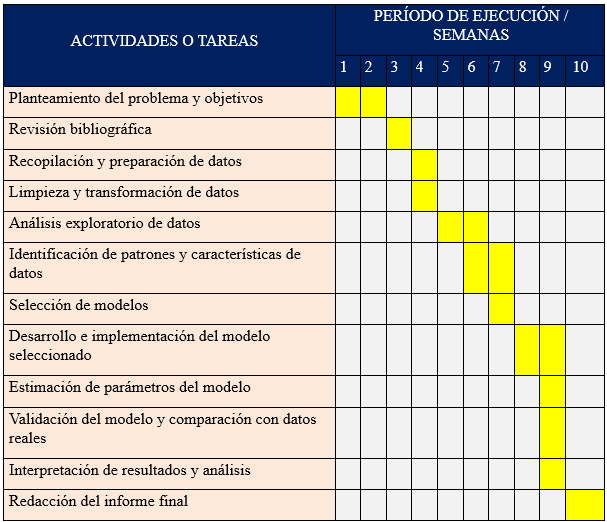
\includegraphics[width=0.9\textwidth]{2/figures/crono_activ.png}
				\caption{Cronograma de actividades}
				\textit{Fuente: Elaboración propia}
				\label{fig8}
			\end{center}	
		\end{figure}
		
		
		\begin{table}[h]
			\centering
			\caption{Presupuesto}
			\begin{tabular}{l|l|l|r}
				\textbf{Recurso} & \textbf{Categoria} & \textbf{Descripción} & \textbf{Costo (Soles)} \\ \hline
				Laptop & Equipo & Equipo de procesamiento del modelo de ML & 3000 \\
				Internet & Servicio & Servicio básico para el uso del estudio & 100\\
				Electricidad  & Servicio & Servicio básico para el uso del estudio  & 200\\
				Python & Software & Lenguaje de programación de alto nivel  & -\\
				Servicio en la nube & Servicio & Alojar backend & 100 \\
				Dominio web & Servicio & Dirección web personalizada & 50 \\
				Mantenimiento Sistema & Servicio & Ajustes, pruebas y monitoreo del sistema & 150 \\
				Almacenamiento nube & Servicio & Espacio virtual para respaldos del proyecto & 50 \\
				 \hline
			\end{tabular}
			\newline
			\newline
			\textit{Fuente: Elaboración propia}
			\label{tab:widgets}
		\end{table}